
\section{Discrete calculus} \label{sec:discrete_calculus}

We wish to describe the temporal variation of the volume flow rate $Q$ and the head $H$ in a one-dimensional domain. This presents us with a bit of problem when it comes to determining flows in networks as connections between more than two pipes/components aren't one-dimensional. One way to approach this difficulty is by considering a discrete calculus \cite{grady10} formulation for the governing equations.

\subsection{Discrete calculus formulation}\label{subsec:discrete_calculus_steady}

The discrete calculus approach has the advantage of directly using the network structure to calculate the derivatives. In the discrete calculus formulation a network is represented as a graph (1-complex) where the edges (1-cells) represent pipes/components and the nodes (0-cells) represent connections and boundaries. The edges of the graph consist of ordered pairs of nodes which define the orientation of the edge. The boundary of each edge is comprised of the union of nodes and the intersection of any two edges is either empty or a boundary element of both edges. 

Flow passing through an edge in the same direction as its orientation is considered positive while flow in the opposite direction is considered negative. We will consider edges that are oriented but not directed since flow is permitted in both directions. An edge consists of two nodes (labelled $\sigma_1$ and $\sigma_2$) and the orientation may be defined by an ordering of these nodes as the list $\tau = \{ \sigma_1, \sigma_2 \}$. A node is considered to have two orientations ("sourceness" and "sinkness") but by convention all nodes will be given the same orientation, "sourceness", so that the negative end of an edge will not be coherent with the orientation of a node.   

\begin{figure}
\centering
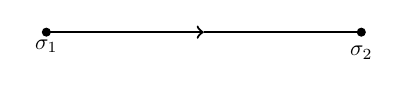
\begin{tikzpicture}[scale=1, every node/.style={scale=0.8}] 
\node[anchor=north] at (3,0) {$\sigma_1$};
\draw[fill=black] (3,0) circle (0.05cm);
\node[anchor=north] at (7,-0.08) {$\sigma_2$};
\draw[fill=black] (7,0) circle (0.05cm);
\draw[thick, ->] (3,0) -- (5,0);
\draw[thick] (5,0) -- (7,0);
\end{tikzpicture} 
\caption{The edge points from $\sigma_1$ to $\sigma_2$; flow from $\sigma_1$ to $\sigma_2$ is considered positive.}
\label{fig:edge_orientation}
\end{figure}

\subsubsection{Incidence matrix}

The structure of a graph (network) may be represented algebraically via an incidence matrix. The incidence matrix $\mathbf{K}^T$ encodes which edges are incident to which nodes in the graph and is defined as 
\begin{align}
K_{ij}=
\begin{cases}
\hspace{0.3cm} 0 \hspace{0.5cm} \text{if } \sigma_j \text{ is not on the boundary of } e_i, \\
+1 \hspace{0.5cm} \text{if } \sigma_j \text{ is coherent with the orientation of } e_i,\\
-1 \hspace{0.5cm} \text{if } \sigma_j \text{ is not coherent with the orientation of } e_i,
\end{cases}
\end{align}
where $e_i$ is the label of an edge in the graph. For a graph the incidence matrix $\mathbf{K}^T$ is an $n \times m$ matrix (where $n$ is the number of nodes and $m$ is the number of edges). For example the graph shown in figure \ref{fig:example_network} has 
\begin{align*}
\mathbf{K} = \begin{bmatrix}
1 & -1 & 0 & 0 & 0 \\
0 & 1 & -1 & 0 & 0 \\
0 & 0 & 1 & -1 & 0 \\
0 & 0 & 1 & 0 & -1 
\end{bmatrix},
\end{align*}
such that the incidence matrix is given by 
\begin{align*}
\mathbf{K}^T = \begin{bmatrix}
1 & 0 & 0 & 0 \\ 
-1 & 1 & 0 & 0 \\
0 & -1 & 1 & 1 \\
0 & 0 & -1 & 0 \\
0 & 0 & 0 & -1
\end{bmatrix}.
\end{align*}

\begin{figure}
\centering
\begin{tikzpicture}[scale=1, every node/.style={scale=0.8}] 
\node[anchor=north] at (3,-0.08) {$\sigma_1$};
\draw[fill=black] (3,0) circle (0.05cm);
\node[anchor=north] at (5,-0.08) {$\sigma_2$};
\draw[fill=black] (5,0) circle (0.05cm);
\node[anchor=north] at (7,-0.08) {$\sigma_3$};
\draw[fill=black] (7,0) circle (0.05cm);
\node[anchor=north] at (9,-0.08) {$\sigma_4$};
\draw[fill=black] (9,0) circle (0.05cm);
\node[anchor=south] at (7,2+0.08) {$\sigma_5$};
\draw[fill=black] (7,2) circle (0.05cm);
\draw[thick, ->] (3,0) -- (4,0);
\draw[thick] (4,0) -- (5,0);
\draw[thick, ->] (5,0) -- (6,0);
\draw[thick] (6,0) -- (7,0);
\draw[thick, ->] (7,0) -- (8,0);
\draw[thick] (8,0) -- (9,0);
\draw[thick, ->] (7,0) -- (7,1);
\draw[thick] (7,1) -- (7,2);
\node[anchor=south] at (4,0.08) {$e_1$};
\node[anchor=south] at (6,0.08) {$e_2$};
\node[anchor=south] at (8,0.08) {$e_3$};
\node[anchor=west] at (7+0.08,1) {$e_4$};
\end{tikzpicture} 
\caption{An example graph with 5 nodes and 4 edges.}
\label{fig:example_network}
\end{figure}

\subsubsection{Chains}

In order to define a domain of integration on the graph we must define a 1-chain. A 1-chain is an $m$-tuple of scalars which assigns a coefficient to each edge where $m$ is the number of distinct edges in the graph. A 1-chain is represented by a column vector of size $m$ with zeros in the entries corresponding to edges not included in the chain. A 1-chain may be viewed as an indicator vector representing a set of edges i.e. $\mathbf{\tau}_1 = [1, 1, 0, 0]^T$ represents the set of edges $\{ e_1, e_2 \}$. Generally a 1-chain $\mathbf{\tau}_1$ may be expressed as 
\begin{align}
\mathbf{\tau}_1 =  \sum_{i=1}^m a^i \mathbf{e}_i, \hspace{0.5cm} a^i \in \mathbb{R},
\end{align}
where the sign of $a^i$ indicates the orientation and $\mathbf{e}_i$ are basis vectors for each edge. 

The incidence matrix $\mathbf{K}^T$ maps 1-chains into their corresponding boundary elements. In other words when $\mathbf{K}^T$ is applied to a 1-chain (edge chain) the result is a 0-chain (node chain) i.e. $\mathbf{\tau}_0 = \mathbf{K}^T \mathbf{\tau}_1$. The chain $\mathbf{\tau}_0$ represents the oriented set of nodes on the boundary of the edges represented by $\mathbf{\tau}_1$. For example for the nodes on the boundary of edges $e_1$ and $e_2$ we have
\begin{align*}
\mathbf{\tau}_0 = \mathbf{K}^T \begin{bmatrix}
1 \\ 1 \\ 0 \\ 0
\end{bmatrix} = \begin{bmatrix}
1 \\ 0 \\ -1 \\ 0 \\ 0
\end{bmatrix},
\end{align*}
which corresponds to the nodes $\sigma_1$ and $\sigma_3$ as expected. For the boundary of the entire graph we have 
\begin{align*}
\mathbf{\tau}_0 = \mathbf{K}^T \begin{bmatrix}
1 \\ 1 \\ 1 \\ 1
\end{bmatrix} = \begin{bmatrix}
1 \\ 0 \\ 1 \\ -1 \\ -1
\end{bmatrix},
\end{align*}
where we see that join points ($\sigma_3$) are considered part of the boundary set. The incidence matrix $\mathbf{K}^T$ provides both a representation of the topology of the graph and the boundary operator. 

\subsubsection{Discrete forms}

We may define a vector space that locally maps 1-chains to scalars at each edge in the graph, called 1-cochains. A 1-cochain may be viewed as a function defined on the domain of edges. We represent a 1-cochain as an $m \times 1$ column vector $\mathbf{c}^1$ where the sign of each coefficient indicates the orientation. We can define integration as the pairing (inner product) of a 1-chain with a 1-cochain,
$[\![ \mathbf{c}^1, \mathbf{\tau}_1 ]\!] = \mathbf{c}^1 \cdot \mathbf{\tau}_1$, producing a scalar quantity. 

\subsubsection{Metric tensor}

Given a set of basic chains $\sigma_i$ we may define a metric tensor 
\begin{align*}
g_{ij} = \langle \sigma_i, \sigma_j \rangle.
\end{align*}
Typically in the discrete setting, the basis set of edges is defined to be orthogonal such that $g_{ij}=0$ for $i \neq j$. The metric tensor thus represented by the $m \times m$ diagonal matrix $\mathbf{G}$ where $\mathbf{G}=\text{diag}(g_{ii})$. Converting a 1-chain into its equivalent 1-cochain consists of a simple scaling of the chain coefficients $\mathbf{c}^1 = \mathbf{G} \mathbf{\tau}_1$.
